%% LyX 2.1.0svn created this file.  For more info, see http://www.lyx.org/.
%% Do not edit unless you really know what you are doing.
\documentclass{article}
\usepackage{graphicx, color}
\newcommand{\hlnumber}[1]{\textcolor[rgb]{0,0,0}{#1}}%
\newcommand{\hlfunctioncall}[1]{\textcolor[rgb]{.5,0,.33}{\textbf{#1}}}%
\newcommand{\hlstring}[1]{\textcolor[rgb]{.6,.6,1}{#1}}%
\newcommand{\hlkeyword}[1]{\textbf{#1}}%
\newcommand{\hlargument}[1]{\textcolor[rgb]{.69,.25,.02}{#1}}%
\newcommand{\hlcomment}[1]{\textcolor[rgb]{.18,.6,.34}{#1}}%
\newcommand{\hlroxygencomment}[1]{\textcolor[rgb]{.44,.48,.7}{#1}}%
\newcommand{\hlformalargs}[1]{\hlargument{#1}}%
\newcommand{\hleqformalargs}[1]{\hlargument{#1}}%
\newcommand{\hlassignement}[1]{\textbf{#1}}%
\newcommand{\hlpackage}[1]{\textcolor[rgb]{.59,.71,.145}{#1}}%
\newcommand{\hlslot}[1]{\textit{#1}}%
\newcommand{\hlsymbol}[1]{#1}%
\newcommand{\hlprompt}[1]{\textcolor[rgb]{.5,.5,.5}{#1}}%

\usepackage{color}%
 
\newsavebox{\hlnormalsizeboxclosebrace}%
\newsavebox{\hlnormalsizeboxopenbrace}%
\newsavebox{\hlnormalsizeboxbackslash}%
\newsavebox{\hlnormalsizeboxlessthan}%
\newsavebox{\hlnormalsizeboxgreaterthan}%
\newsavebox{\hlnormalsizeboxdollar}%
\newsavebox{\hlnormalsizeboxunderscore}%
\newsavebox{\hlnormalsizeboxand}%
\newsavebox{\hlnormalsizeboxhash}%
\newsavebox{\hlnormalsizeboxat}%
\newsavebox{\hlnormalsizeboxpercent}% 
\newsavebox{\hlnormalsizeboxhat}%
\newsavebox{\hlnormalsizeboxsinglequote}%
\newsavebox{\hlnormalsizeboxbacktick}%

\setbox\hlnormalsizeboxopenbrace=\hbox{\begin{normalsize}\verb.{.\end{normalsize}}%
\setbox\hlnormalsizeboxclosebrace=\hbox{\begin{normalsize}\verb.}.\end{normalsize}}%
\setbox\hlnormalsizeboxlessthan=\hbox{\begin{normalsize}\verb.<.\end{normalsize}}%
\setbox\hlnormalsizeboxdollar=\hbox{\begin{normalsize}\verb.$.\end{normalsize}}%
\setbox\hlnormalsizeboxunderscore=\hbox{\begin{normalsize}\verb._.\end{normalsize}}%
\setbox\hlnormalsizeboxand=\hbox{\begin{normalsize}\verb.&.\end{normalsize}}%
\setbox\hlnormalsizeboxhash=\hbox{\begin{normalsize}\verb.#.\end{normalsize}}%
\setbox\hlnormalsizeboxat=\hbox{\begin{normalsize}\verb.@.\end{normalsize}}%
\setbox\hlnormalsizeboxbackslash=\hbox{\begin{normalsize}\verb.\.\end{normalsize}}%
\setbox\hlnormalsizeboxgreaterthan=\hbox{\begin{normalsize}\verb.>.\end{normalsize}}%
\setbox\hlnormalsizeboxpercent=\hbox{\begin{normalsize}\verb.%.\end{normalsize}}%
\setbox\hlnormalsizeboxhat=\hbox{\begin{normalsize}\verb.^.\end{normalsize}}%
\setbox\hlnormalsizeboxsinglequote=\hbox{\begin{normalsize}\verb.'.\end{normalsize}}%
\setbox\hlnormalsizeboxbacktick=\hbox{\begin{normalsize}\verb.`.\end{normalsize}}%
\setbox\hlnormalsizeboxhat=\hbox{\begin{normalsize}\verb.^.\end{normalsize}}%



\newsavebox{\hltinyboxclosebrace}%
\newsavebox{\hltinyboxopenbrace}%
\newsavebox{\hltinyboxbackslash}%
\newsavebox{\hltinyboxlessthan}%
\newsavebox{\hltinyboxgreaterthan}%
\newsavebox{\hltinyboxdollar}%
\newsavebox{\hltinyboxunderscore}%
\newsavebox{\hltinyboxand}%
\newsavebox{\hltinyboxhash}%
\newsavebox{\hltinyboxat}%
\newsavebox{\hltinyboxpercent}% 
\newsavebox{\hltinyboxhat}%
\newsavebox{\hltinyboxsinglequote}%
\newsavebox{\hltinyboxbacktick}%

\setbox\hltinyboxopenbrace=\hbox{\begin{tiny}\verb.{.\end{tiny}}%
\setbox\hltinyboxclosebrace=\hbox{\begin{tiny}\verb.}.\end{tiny}}%
\setbox\hltinyboxlessthan=\hbox{\begin{tiny}\verb.<.\end{tiny}}%
\setbox\hltinyboxdollar=\hbox{\begin{tiny}\verb.$.\end{tiny}}%
\setbox\hltinyboxunderscore=\hbox{\begin{tiny}\verb._.\end{tiny}}%
\setbox\hltinyboxand=\hbox{\begin{tiny}\verb.&.\end{tiny}}%
\setbox\hltinyboxhash=\hbox{\begin{tiny}\verb.#.\end{tiny}}%
\setbox\hltinyboxat=\hbox{\begin{tiny}\verb.@.\end{tiny}}%
\setbox\hltinyboxbackslash=\hbox{\begin{tiny}\verb.\.\end{tiny}}%
\setbox\hltinyboxgreaterthan=\hbox{\begin{tiny}\verb.>.\end{tiny}}%
\setbox\hltinyboxpercent=\hbox{\begin{tiny}\verb.%.\end{tiny}}%
\setbox\hltinyboxhat=\hbox{\begin{tiny}\verb.^.\end{tiny}}%
\setbox\hltinyboxsinglequote=\hbox{\begin{tiny}\verb.'.\end{tiny}}%
\setbox\hltinyboxbacktick=\hbox{\begin{tiny}\verb.`.\end{tiny}}%
\setbox\hltinyboxhat=\hbox{\begin{tiny}\verb.^.\end{tiny}}%



\newsavebox{\hlscriptsizeboxclosebrace}%
\newsavebox{\hlscriptsizeboxopenbrace}%
\newsavebox{\hlscriptsizeboxbackslash}%
\newsavebox{\hlscriptsizeboxlessthan}%
\newsavebox{\hlscriptsizeboxgreaterthan}%
\newsavebox{\hlscriptsizeboxdollar}%
\newsavebox{\hlscriptsizeboxunderscore}%
\newsavebox{\hlscriptsizeboxand}%
\newsavebox{\hlscriptsizeboxhash}%
\newsavebox{\hlscriptsizeboxat}%
\newsavebox{\hlscriptsizeboxpercent}% 
\newsavebox{\hlscriptsizeboxhat}%
\newsavebox{\hlscriptsizeboxsinglequote}%
\newsavebox{\hlscriptsizeboxbacktick}%

\setbox\hlscriptsizeboxopenbrace=\hbox{\begin{scriptsize}\verb.{.\end{scriptsize}}%
\setbox\hlscriptsizeboxclosebrace=\hbox{\begin{scriptsize}\verb.}.\end{scriptsize}}%
\setbox\hlscriptsizeboxlessthan=\hbox{\begin{scriptsize}\verb.<.\end{scriptsize}}%
\setbox\hlscriptsizeboxdollar=\hbox{\begin{scriptsize}\verb.$.\end{scriptsize}}%
\setbox\hlscriptsizeboxunderscore=\hbox{\begin{scriptsize}\verb._.\end{scriptsize}}%
\setbox\hlscriptsizeboxand=\hbox{\begin{scriptsize}\verb.&.\end{scriptsize}}%
\setbox\hlscriptsizeboxhash=\hbox{\begin{scriptsize}\verb.#.\end{scriptsize}}%
\setbox\hlscriptsizeboxat=\hbox{\begin{scriptsize}\verb.@.\end{scriptsize}}%
\setbox\hlscriptsizeboxbackslash=\hbox{\begin{scriptsize}\verb.\.\end{scriptsize}}%
\setbox\hlscriptsizeboxgreaterthan=\hbox{\begin{scriptsize}\verb.>.\end{scriptsize}}%
\setbox\hlscriptsizeboxpercent=\hbox{\begin{scriptsize}\verb.%.\end{scriptsize}}%
\setbox\hlscriptsizeboxhat=\hbox{\begin{scriptsize}\verb.^.\end{scriptsize}}%
\setbox\hlscriptsizeboxsinglequote=\hbox{\begin{scriptsize}\verb.'.\end{scriptsize}}%
\setbox\hlscriptsizeboxbacktick=\hbox{\begin{scriptsize}\verb.`.\end{scriptsize}}%
\setbox\hlscriptsizeboxhat=\hbox{\begin{scriptsize}\verb.^.\end{scriptsize}}%



\newsavebox{\hlfootnotesizeboxclosebrace}%
\newsavebox{\hlfootnotesizeboxopenbrace}%
\newsavebox{\hlfootnotesizeboxbackslash}%
\newsavebox{\hlfootnotesizeboxlessthan}%
\newsavebox{\hlfootnotesizeboxgreaterthan}%
\newsavebox{\hlfootnotesizeboxdollar}%
\newsavebox{\hlfootnotesizeboxunderscore}%
\newsavebox{\hlfootnotesizeboxand}%
\newsavebox{\hlfootnotesizeboxhash}%
\newsavebox{\hlfootnotesizeboxat}%
\newsavebox{\hlfootnotesizeboxpercent}% 
\newsavebox{\hlfootnotesizeboxhat}%
\newsavebox{\hlfootnotesizeboxsinglequote}%
\newsavebox{\hlfootnotesizeboxbacktick}%

\setbox\hlfootnotesizeboxopenbrace=\hbox{\begin{footnotesize}\verb.{.\end{footnotesize}}%
\setbox\hlfootnotesizeboxclosebrace=\hbox{\begin{footnotesize}\verb.}.\end{footnotesize}}%
\setbox\hlfootnotesizeboxlessthan=\hbox{\begin{footnotesize}\verb.<.\end{footnotesize}}%
\setbox\hlfootnotesizeboxdollar=\hbox{\begin{footnotesize}\verb.$.\end{footnotesize}}%
\setbox\hlfootnotesizeboxunderscore=\hbox{\begin{footnotesize}\verb._.\end{footnotesize}}%
\setbox\hlfootnotesizeboxand=\hbox{\begin{footnotesize}\verb.&.\end{footnotesize}}%
\setbox\hlfootnotesizeboxhash=\hbox{\begin{footnotesize}\verb.#.\end{footnotesize}}%
\setbox\hlfootnotesizeboxat=\hbox{\begin{footnotesize}\verb.@.\end{footnotesize}}%
\setbox\hlfootnotesizeboxbackslash=\hbox{\begin{footnotesize}\verb.\.\end{footnotesize}}%
\setbox\hlfootnotesizeboxgreaterthan=\hbox{\begin{footnotesize}\verb.>.\end{footnotesize}}%
\setbox\hlfootnotesizeboxpercent=\hbox{\begin{footnotesize}\verb.%.\end{footnotesize}}%
\setbox\hlfootnotesizeboxhat=\hbox{\begin{footnotesize}\verb.^.\end{footnotesize}}%
\setbox\hlfootnotesizeboxsinglequote=\hbox{\begin{footnotesize}\verb.'.\end{footnotesize}}%
\setbox\hlfootnotesizeboxbacktick=\hbox{\begin{footnotesize}\verb.`.\end{footnotesize}}%
\setbox\hlfootnotesizeboxhat=\hbox{\begin{footnotesize}\verb.^.\end{footnotesize}}%



\newsavebox{\hlsmallboxclosebrace}%
\newsavebox{\hlsmallboxopenbrace}%
\newsavebox{\hlsmallboxbackslash}%
\newsavebox{\hlsmallboxlessthan}%
\newsavebox{\hlsmallboxgreaterthan}%
\newsavebox{\hlsmallboxdollar}%
\newsavebox{\hlsmallboxunderscore}%
\newsavebox{\hlsmallboxand}%
\newsavebox{\hlsmallboxhash}%
\newsavebox{\hlsmallboxat}%
\newsavebox{\hlsmallboxpercent}% 
\newsavebox{\hlsmallboxhat}%
\newsavebox{\hlsmallboxsinglequote}%
\newsavebox{\hlsmallboxbacktick}%

\setbox\hlsmallboxopenbrace=\hbox{\begin{small}\verb.{.\end{small}}%
\setbox\hlsmallboxclosebrace=\hbox{\begin{small}\verb.}.\end{small}}%
\setbox\hlsmallboxlessthan=\hbox{\begin{small}\verb.<.\end{small}}%
\setbox\hlsmallboxdollar=\hbox{\begin{small}\verb.$.\end{small}}%
\setbox\hlsmallboxunderscore=\hbox{\begin{small}\verb._.\end{small}}%
\setbox\hlsmallboxand=\hbox{\begin{small}\verb.&.\end{small}}%
\setbox\hlsmallboxhash=\hbox{\begin{small}\verb.#.\end{small}}%
\setbox\hlsmallboxat=\hbox{\begin{small}\verb.@.\end{small}}%
\setbox\hlsmallboxbackslash=\hbox{\begin{small}\verb.\.\end{small}}%
\setbox\hlsmallboxgreaterthan=\hbox{\begin{small}\verb.>.\end{small}}%
\setbox\hlsmallboxpercent=\hbox{\begin{small}\verb.%.\end{small}}%
\setbox\hlsmallboxhat=\hbox{\begin{small}\verb.^.\end{small}}%
\setbox\hlsmallboxsinglequote=\hbox{\begin{small}\verb.'.\end{small}}%
\setbox\hlsmallboxbacktick=\hbox{\begin{small}\verb.`.\end{small}}%
\setbox\hlsmallboxhat=\hbox{\begin{small}\verb.^.\end{small}}%



\newsavebox{\hllargeboxclosebrace}%
\newsavebox{\hllargeboxopenbrace}%
\newsavebox{\hllargeboxbackslash}%
\newsavebox{\hllargeboxlessthan}%
\newsavebox{\hllargeboxgreaterthan}%
\newsavebox{\hllargeboxdollar}%
\newsavebox{\hllargeboxunderscore}%
\newsavebox{\hllargeboxand}%
\newsavebox{\hllargeboxhash}%
\newsavebox{\hllargeboxat}%
\newsavebox{\hllargeboxpercent}% 
\newsavebox{\hllargeboxhat}%
\newsavebox{\hllargeboxsinglequote}%
\newsavebox{\hllargeboxbacktick}%

\setbox\hllargeboxopenbrace=\hbox{\begin{large}\verb.{.\end{large}}%
\setbox\hllargeboxclosebrace=\hbox{\begin{large}\verb.}.\end{large}}%
\setbox\hllargeboxlessthan=\hbox{\begin{large}\verb.<.\end{large}}%
\setbox\hllargeboxdollar=\hbox{\begin{large}\verb.$.\end{large}}%
\setbox\hllargeboxunderscore=\hbox{\begin{large}\verb._.\end{large}}%
\setbox\hllargeboxand=\hbox{\begin{large}\verb.&.\end{large}}%
\setbox\hllargeboxhash=\hbox{\begin{large}\verb.#.\end{large}}%
\setbox\hllargeboxat=\hbox{\begin{large}\verb.@.\end{large}}%
\setbox\hllargeboxbackslash=\hbox{\begin{large}\verb.\.\end{large}}%
\setbox\hllargeboxgreaterthan=\hbox{\begin{large}\verb.>.\end{large}}%
\setbox\hllargeboxpercent=\hbox{\begin{large}\verb.%.\end{large}}%
\setbox\hllargeboxhat=\hbox{\begin{large}\verb.^.\end{large}}%
\setbox\hllargeboxsinglequote=\hbox{\begin{large}\verb.'.\end{large}}%
\setbox\hllargeboxbacktick=\hbox{\begin{large}\verb.`.\end{large}}%
\setbox\hllargeboxhat=\hbox{\begin{large}\verb.^.\end{large}}%



\newsavebox{\hlLargeboxclosebrace}%
\newsavebox{\hlLargeboxopenbrace}%
\newsavebox{\hlLargeboxbackslash}%
\newsavebox{\hlLargeboxlessthan}%
\newsavebox{\hlLargeboxgreaterthan}%
\newsavebox{\hlLargeboxdollar}%
\newsavebox{\hlLargeboxunderscore}%
\newsavebox{\hlLargeboxand}%
\newsavebox{\hlLargeboxhash}%
\newsavebox{\hlLargeboxat}%
\newsavebox{\hlLargeboxpercent}% 
\newsavebox{\hlLargeboxhat}%
\newsavebox{\hlLargeboxsinglequote}%
\newsavebox{\hlLargeboxbacktick}%

\setbox\hlLargeboxopenbrace=\hbox{\begin{Large}\verb.{.\end{Large}}%
\setbox\hlLargeboxclosebrace=\hbox{\begin{Large}\verb.}.\end{Large}}%
\setbox\hlLargeboxlessthan=\hbox{\begin{Large}\verb.<.\end{Large}}%
\setbox\hlLargeboxdollar=\hbox{\begin{Large}\verb.$.\end{Large}}%
\setbox\hlLargeboxunderscore=\hbox{\begin{Large}\verb._.\end{Large}}%
\setbox\hlLargeboxand=\hbox{\begin{Large}\verb.&.\end{Large}}%
\setbox\hlLargeboxhash=\hbox{\begin{Large}\verb.#.\end{Large}}%
\setbox\hlLargeboxat=\hbox{\begin{Large}\verb.@.\end{Large}}%
\setbox\hlLargeboxbackslash=\hbox{\begin{Large}\verb.\.\end{Large}}%
\setbox\hlLargeboxgreaterthan=\hbox{\begin{Large}\verb.>.\end{Large}}%
\setbox\hlLargeboxpercent=\hbox{\begin{Large}\verb.%.\end{Large}}%
\setbox\hlLargeboxhat=\hbox{\begin{Large}\verb.^.\end{Large}}%
\setbox\hlLargeboxsinglequote=\hbox{\begin{Large}\verb.'.\end{Large}}%
\setbox\hlLargeboxbacktick=\hbox{\begin{Large}\verb.`.\end{Large}}%
\setbox\hlLargeboxhat=\hbox{\begin{Large}\verb.^.\end{Large}}%



\newsavebox{\hlLARGEboxclosebrace}%
\newsavebox{\hlLARGEboxopenbrace}%
\newsavebox{\hlLARGEboxbackslash}%
\newsavebox{\hlLARGEboxlessthan}%
\newsavebox{\hlLARGEboxgreaterthan}%
\newsavebox{\hlLARGEboxdollar}%
\newsavebox{\hlLARGEboxunderscore}%
\newsavebox{\hlLARGEboxand}%
\newsavebox{\hlLARGEboxhash}%
\newsavebox{\hlLARGEboxat}%
\newsavebox{\hlLARGEboxpercent}% 
\newsavebox{\hlLARGEboxhat}%
\newsavebox{\hlLARGEboxsinglequote}%
\newsavebox{\hlLARGEboxbacktick}%

\setbox\hlLARGEboxopenbrace=\hbox{\begin{LARGE}\verb.{.\end{LARGE}}%
\setbox\hlLARGEboxclosebrace=\hbox{\begin{LARGE}\verb.}.\end{LARGE}}%
\setbox\hlLARGEboxlessthan=\hbox{\begin{LARGE}\verb.<.\end{LARGE}}%
\setbox\hlLARGEboxdollar=\hbox{\begin{LARGE}\verb.$.\end{LARGE}}%
\setbox\hlLARGEboxunderscore=\hbox{\begin{LARGE}\verb._.\end{LARGE}}%
\setbox\hlLARGEboxand=\hbox{\begin{LARGE}\verb.&.\end{LARGE}}%
\setbox\hlLARGEboxhash=\hbox{\begin{LARGE}\verb.#.\end{LARGE}}%
\setbox\hlLARGEboxat=\hbox{\begin{LARGE}\verb.@.\end{LARGE}}%
\setbox\hlLARGEboxbackslash=\hbox{\begin{LARGE}\verb.\.\end{LARGE}}%
\setbox\hlLARGEboxgreaterthan=\hbox{\begin{LARGE}\verb.>.\end{LARGE}}%
\setbox\hlLARGEboxpercent=\hbox{\begin{LARGE}\verb.%.\end{LARGE}}%
\setbox\hlLARGEboxhat=\hbox{\begin{LARGE}\verb.^.\end{LARGE}}%
\setbox\hlLARGEboxsinglequote=\hbox{\begin{LARGE}\verb.'.\end{LARGE}}%
\setbox\hlLARGEboxbacktick=\hbox{\begin{LARGE}\verb.`.\end{LARGE}}%
\setbox\hlLARGEboxhat=\hbox{\begin{LARGE}\verb.^.\end{LARGE}}%



\newsavebox{\hlhugeboxclosebrace}%
\newsavebox{\hlhugeboxopenbrace}%
\newsavebox{\hlhugeboxbackslash}%
\newsavebox{\hlhugeboxlessthan}%
\newsavebox{\hlhugeboxgreaterthan}%
\newsavebox{\hlhugeboxdollar}%
\newsavebox{\hlhugeboxunderscore}%
\newsavebox{\hlhugeboxand}%
\newsavebox{\hlhugeboxhash}%
\newsavebox{\hlhugeboxat}%
\newsavebox{\hlhugeboxpercent}% 
\newsavebox{\hlhugeboxhat}%
\newsavebox{\hlhugeboxsinglequote}%
\newsavebox{\hlhugeboxbacktick}%

\setbox\hlhugeboxopenbrace=\hbox{\begin{huge}\verb.{.\end{huge}}%
\setbox\hlhugeboxclosebrace=\hbox{\begin{huge}\verb.}.\end{huge}}%
\setbox\hlhugeboxlessthan=\hbox{\begin{huge}\verb.<.\end{huge}}%
\setbox\hlhugeboxdollar=\hbox{\begin{huge}\verb.$.\end{huge}}%
\setbox\hlhugeboxunderscore=\hbox{\begin{huge}\verb._.\end{huge}}%
\setbox\hlhugeboxand=\hbox{\begin{huge}\verb.&.\end{huge}}%
\setbox\hlhugeboxhash=\hbox{\begin{huge}\verb.#.\end{huge}}%
\setbox\hlhugeboxat=\hbox{\begin{huge}\verb.@.\end{huge}}%
\setbox\hlhugeboxbackslash=\hbox{\begin{huge}\verb.\.\end{huge}}%
\setbox\hlhugeboxgreaterthan=\hbox{\begin{huge}\verb.>.\end{huge}}%
\setbox\hlhugeboxpercent=\hbox{\begin{huge}\verb.%.\end{huge}}%
\setbox\hlhugeboxhat=\hbox{\begin{huge}\verb.^.\end{huge}}%
\setbox\hlhugeboxsinglequote=\hbox{\begin{huge}\verb.'.\end{huge}}%
\setbox\hlhugeboxbacktick=\hbox{\begin{huge}\verb.`.\end{huge}}%
\setbox\hlhugeboxhat=\hbox{\begin{huge}\verb.^.\end{huge}}%



\newsavebox{\hlHugeboxclosebrace}%
\newsavebox{\hlHugeboxopenbrace}%
\newsavebox{\hlHugeboxbackslash}%
\newsavebox{\hlHugeboxlessthan}%
\newsavebox{\hlHugeboxgreaterthan}%
\newsavebox{\hlHugeboxdollar}%
\newsavebox{\hlHugeboxunderscore}%
\newsavebox{\hlHugeboxand}%
\newsavebox{\hlHugeboxhash}%
\newsavebox{\hlHugeboxat}%
\newsavebox{\hlHugeboxpercent}% 
\newsavebox{\hlHugeboxhat}%
\newsavebox{\hlHugeboxsinglequote}%
\newsavebox{\hlHugeboxbacktick}%

\setbox\hlHugeboxopenbrace=\hbox{\begin{Huge}\verb.{.\end{Huge}}%
\setbox\hlHugeboxclosebrace=\hbox{\begin{Huge}\verb.}.\end{Huge}}%
\setbox\hlHugeboxlessthan=\hbox{\begin{Huge}\verb.<.\end{Huge}}%
\setbox\hlHugeboxdollar=\hbox{\begin{Huge}\verb.$.\end{Huge}}%
\setbox\hlHugeboxunderscore=\hbox{\begin{Huge}\verb._.\end{Huge}}%
\setbox\hlHugeboxand=\hbox{\begin{Huge}\verb.&.\end{Huge}}%
\setbox\hlHugeboxhash=\hbox{\begin{Huge}\verb.#.\end{Huge}}%
\setbox\hlHugeboxat=\hbox{\begin{Huge}\verb.@.\end{Huge}}%
\setbox\hlHugeboxbackslash=\hbox{\begin{Huge}\verb.\.\end{Huge}}%
\setbox\hlHugeboxgreaterthan=\hbox{\begin{Huge}\verb.>.\end{Huge}}%
\setbox\hlHugeboxpercent=\hbox{\begin{Huge}\verb.%.\end{Huge}}%
\setbox\hlHugeboxhat=\hbox{\begin{Huge}\verb.^.\end{Huge}}%
\setbox\hlHugeboxsinglequote=\hbox{\begin{Huge}\verb.'.\end{Huge}}%
\setbox\hlHugeboxbacktick=\hbox{\begin{Huge}\verb.`.\end{Huge}}%
\setbox\hlHugeboxhat=\hbox{\begin{Huge}\verb.^.\end{Huge}}%
 

\def\urltilda{\kern -.15em\lower .7ex\hbox{\~{}}\kern .04em}%

\newcommand{\hlstd}[1]{\textcolor[rgb]{0,0,0}{#1}}%
\newcommand{\hlnum}[1]{\textcolor[rgb]{0.16,0.16,1}{#1}}
\newcommand{\hlesc}[1]{\textcolor[rgb]{1,0,1}{#1}}
\newcommand{\hlstr}[1]{\textcolor[rgb]{1,0,0}{#1}}
\newcommand{\hldstr}[1]{\textcolor[rgb]{0.51,0.51,0}{#1}}
\newcommand{\hlslc}[1]{\textcolor[rgb]{0.51,0.51,0.51}{\it{#1}}}
\newcommand{\hlcom}[1]{\textcolor[rgb]{0.51,0.51,0.51}{\it{#1}}}
\newcommand{\hldir}[1]{\textcolor[rgb]{0,0.51,0}{#1}}
\newcommand{\hlsym}[1]{\textcolor[rgb]{0,0,0}{#1}}
\newcommand{\hlline}[1]{\textcolor[rgb]{0.33,0.33,0.33}{#1}}
\newcommand{\hlkwa}[1]{\textcolor[rgb]{0,0,0}{\bf{#1}}}
\newcommand{\hlkwb}[1]{\textcolor[rgb]{0.51,0,0}{#1}}
\newcommand{\hlkwc}[1]{\textcolor[rgb]{0,0,0}{\bf{#1}}}
\newcommand{\hlkwd}[1]{\textcolor[rgb]{0,0,0.51}{#1}}

\definecolor{fgcolor}{rgb}{0,0,0}
\usepackage{framed}
\makeatletter
\newenvironment{kframe}{%
 \def\FrameCommand##1{\hskip\@totalleftmargin \hskip-\fboxsep
 \colorbox{shadecolor}{##1}\hskip-\fboxsep
     % There is no \@totalrightmargin, so:
     \hskip-\linewidth \hskip-\@totalleftmargin \hskip\columnwidth}%
 \MakeFramed {\advance\hsize-\width
   \@totalleftmargin\z@ \linewidth\hsize
   \@setminipage}}%
 {\par\unskip\endMakeFramed}
\makeatother

\newenvironment{knitrout}{}{} % an empty environment to be redefined in TeX

\usepackage[sc]{mathpazo}
\usepackage[T1]{fontenc}
\usepackage{geometry}
\usepackage{amssymb}
\usepackage{amsmath}
\geometry{verbose,tmargin=2.5cm,bmargin=2.5cm,lmargin=2.5cm,rmargin=2.5cm}
\setcounter{secnumdepth}{2}
\setcounter{tocdepth}{2}
\usepackage{url}
\usepackage[unicode=true,pdfusetitle,
 bookmarks=true,bookmarksnumbered=true,bookmarksopen=true,bookmarksopenlevel=2,
 breaklinks=false,pdfborder={0 0 1},backref=false,colorlinks=false]
 {hyperref}
\hypersetup{
 pdfstartview={XYZ null null 1}}
%\usepackage{breakurl}

\makeatletter
%%%%%%%%%%%%%%%%%%%%%%%%%%%%%% User specified LaTeX commands.
\renewcommand{\textfraction}{0.05}
\renewcommand{\topfraction}{0.8}
\renewcommand{\bottomfraction}{0.8}
\renewcommand{\floatpagefraction}{0.75}

\makeatother

\begin{document}

%% still can't get paths to work ...
% 




\begin{center}
  {\bf \Large Homework 3, Statistical Rethinking}\\
\vspace{12pt}
   {\large Jaime Ashander}
\end{center}



\subsection*{Problem 1}
\label{problem1}


\begin{knitrout}
\definecolor{shadecolor}{rgb}{.97, .97, .97}{\color{fgcolor}\begin{kframe}
\begin{flushleft}
\ttfamily\noindent
\hlfunctioncall{data}\hlkeyword{(}\hlsymbol{Howell1}\hlkeyword{)}\hspace*{\fill}\\
\hlstd{}\hlsymbol{d2}{\ }\hlassignement{\usebox{\hlnormalsizeboxlessthan}-}{\ }\hlsymbol{Howell1}\hlkeyword{[}\hlsymbol{Howell1}\hlkeyword{\usebox{\hlnormalsizeboxdollar}}\hlsymbol{age}{\ }\hlkeyword{\usebox{\hlnormalsizeboxgreaterthan}=}{\ }\hlnumber{18}\hlkeyword{,}{\ }\hlkeyword{]}\mbox{}
\normalfont
\end{flushleft}
\end{kframe}}
\end{knitrout}


Model the relationship between height $h_i$ and weight $w_i$ as
\[
h_i  ~ {\rm Normal}\left ( \mu_i, \sigma \right). 
\]

with $\mu_i = \alpha + \beta w_i$

Note that $h_i$ is column `height` and $w_i$ is column `weight` in the data frame `d2`. 

\begin{knitrout}
\definecolor{shadecolor}{rgb}{.97, .97, .97}{\color{fgcolor}\begin{kframe}
\begin{flushleft}
\ttfamily\noindent
\hlsymbol{mle.hw}{\ }\hlassignement{\usebox{\hlnormalsizeboxlessthan}-}{\ }\hlfunctioncall{mle2}\hlkeyword{(}\hlsymbol{height}{\ }\hlkeyword{\urltilda{}}{\ }\hlfunctioncall{dnorm}\hlkeyword{(}\hlargument{mean}{\ }\hlargument{=}{\ }\hlsymbol{alpha}{\ }\hlkeyword{+}{\ }\hlsymbol{beta}{\ }\hlkeyword{*}{\ }\hlsymbol{weight}\hlkeyword{,}\hspace*{\fill}\\
\hlstd{}{\ }{\ }{\ }{\ }\hlargument{sd}{\ }\hlargument{=}{\ }\hlsymbol{sigma}\hlkeyword{)}\hlkeyword{,}{\ }\hlargument{data}{\ }\hlargument{=}{\ }\hlsymbol{d2}\hlkeyword{,}{\ }\hlargument{start}{\ }\hlargument{=}{\ }\hlfunctioncall{list}\hlkeyword{(}\hlargument{alpha}{\ }\hlargument{=}{\ }\hlfunctioncall{mean}\hlkeyword{(}\hlsymbol{d2}\hlkeyword{\usebox{\hlnormalsizeboxdollar}}\hlsymbol{height}\hlkeyword{)}\hlkeyword{,}{\ }\hlargument{beta}{\ }\hlargument{=}{\ }\hlnumber{0}\hlkeyword{,}\hspace*{\fill}\\
\hlstd{}{\ }{\ }{\ }{\ }\hlargument{sigma}{\ }\hlargument{=}{\ }\hlfunctioncall{sd}\hlkeyword{(}\hlsymbol{d2}\hlkeyword{\usebox{\hlnormalsizeboxdollar}}\hlsymbol{height}\hlkeyword{)}\hlkeyword{)}\hlkeyword{)}\mbox{}
\normalfont
\end{flushleft}
\begin{verbatim}
## Warning message: NaNs produced
\end{verbatim}
\begin{verbatim}
## Warning message: NaNs produced
\end{verbatim}
\begin{verbatim}
## Warning message: NaNs produced
\end{verbatim}
\begin{verbatim}
## Warning message: NaNs produced
\end{verbatim}
\begin{verbatim}
## Warning message: NaNs produced
\end{verbatim}
\begin{flushleft}
\ttfamily\noindent
\hlsymbol{known.weights}{\ }\hlassignement{\usebox{\hlnormalsizeboxlessthan}-}{\ }\hlfunctioncall{c}\hlkeyword{(}\hlnumber{46.95}\hlkeyword{,}{\ }\hlnumber{43.72}\hlkeyword{,}{\ }\hlnumber{64.78}\hlkeyword{,}{\ }\hlnumber{32.59}\hlkeyword{,}{\ }\hlnumber{54.63}\hlkeyword{)}\hspace*{\fill}\\
\hlstd{}\hlsymbol{post.samples}{\ }\hlassignement{\usebox{\hlnormalsizeboxlessthan}-}{\ }\hlfunctioncall{as.data.frame}\hlkeyword{(}\hlfunctioncall{mvrnorm}\hlkeyword{(}\hlfunctioncall{length}\hlkeyword{(}\hlsymbol{d2}\hlkeyword{\usebox{\hlnormalsizeboxdollar}}\hlsymbol{height}\hlkeyword{)}\hlkeyword{,}\hspace*{\fill}\\
\hlstd{}{\ }{\ }{\ }{\ }\hlargument{mu}{\ }\hlargument{=}{\ }\hlfunctioncall{coef}\hlkeyword{(}\hlsymbol{mle.hw}\hlkeyword{)}\hlkeyword{,}{\ }\hlargument{Sigma}{\ }\hlargument{=}{\ }\hlfunctioncall{vcov}\hlkeyword{(}\hlsymbol{mle.hw}\hlkeyword{)}\hlkeyword{)}\hlkeyword{)}\hspace*{\fill}\\
\hlstd{}\hlsymbol{Pred.mean}{\ }\hlassignement{\usebox{\hlnormalsizeboxlessthan}-}{\ }\hlkeyword{function}\hlkeyword{(}\hlformalargs{x}\hlkeyword{)}{\ }\hlkeyword{\usebox{\hlnormalsizeboxopenbrace}}\hspace*{\fill}\\
\hlstd{}{\ }{\ }{\ }{\ }\hlsymbol{ret}{\ }\hlassignement{\usebox{\hlnormalsizeboxlessthan}-}{\ }\hlfunctioncall{coef}\hlkeyword{(}\hlsymbol{mle.hw}\hlkeyword{)}\hlkeyword{[}\hlstring{"alpha"}\hlkeyword{]}{\ }\hlkeyword{+}{\ }\hlfunctioncall{coef}\hlkeyword{(}\hlsymbol{mle.hw}\hlkeyword{)}\hlkeyword{[}\hlstring{"beta"}\hlkeyword{]}{\ }\hlkeyword{*}{\ }\hlsymbol{x}\hspace*{\fill}\\
\hlstd{}{\ }{\ }{\ }{\ }\hlfunctioncall{names}\hlkeyword{(}\hlsymbol{ret}\hlkeyword{)}{\ }\hlassignement{\usebox{\hlnormalsizeboxlessthan}-}{\ }\hlfunctioncall{c}\hlkeyword{(}\hlstring{""}\hlkeyword{)}\hspace*{\fill}\\
\hlstd{}{\ }{\ }{\ }{\ }\hlsymbol{ret}\hspace*{\fill}\\
\hlstd{}\hlkeyword{\usebox{\hlnormalsizeboxclosebrace}}\hspace*{\fill}\\
\hlstd{}\hlsymbol{height.CI}{\ }\hlassignement{\usebox{\hlnormalsizeboxlessthan}-}{\ }\hlfunctioncall{sapply}\hlkeyword{(}\hlsymbol{known.weights}\hlkeyword{,}{\ }\hlkeyword{function}\hlkeyword{(}\hlformalargs{x}\hlkeyword{)}{\ }\hlkeyword{\usebox{\hlnormalsizeboxopenbrace}}\hspace*{\fill}\\
\hlstd{}{\ }{\ }{\ }{\ }\hlfunctioncall{HPDI}\hlkeyword{(}\hlsymbol{post.samples}\hlkeyword{\usebox{\hlnormalsizeboxdollar}}\hlsymbol{alpha}{\ }\hlkeyword{+}{\ }\hlsymbol{post.samples}\hlkeyword{\usebox{\hlnormalsizeboxdollar}}\hlsymbol{beta}{\ }\hlkeyword{*}{\ }\hlsymbol{x}\hlkeyword{)}\hspace*{\fill}\\
\hlstd{}\hlkeyword{\usebox{\hlnormalsizeboxclosebrace}}\hlkeyword{)}\hspace*{\fill}\\
\hlstd{}\hlsymbol{height.mean}{\ }\hlassignement{\usebox{\hlnormalsizeboxlessthan}-}{\ }\hlfunctioncall{sapply}\hlkeyword{(}\hlsymbol{known.weights}\hlkeyword{,}{\ }\hlsymbol{Pred.mean}\hlkeyword{)}\hspace*{\fill}\\
\hlstd{}\hlsymbol{height.table}{\ }\hlassignement{\usebox{\hlnormalsizeboxlessthan}-}{\ }\hlfunctioncall{cbind}\hlkeyword{(}\hlargument{individual}{\ }\hlargument{=}{\ }\hlnumber{1}\hlkeyword{:}\hlnumber{5}\hlkeyword{,}{\ }\hlsymbol{known.weights}\hlkeyword{,}{\ }\hlargument{expected.height}{\ }\hlargument{=}{\ }\hlsymbol{height.mean}\hlkeyword{,}\hspace*{\fill}\\
\hlstd{}{\ }{\ }{\ }{\ }\hlargument{lower.90}{\ }\hlargument{=}{\ }\hlsymbol{height.CI}\hlkeyword{[}\hlnumber{1}\hlkeyword{,}{\ }\hlkeyword{]}\hlkeyword{,}{\ }\hlargument{upper.90}{\ }\hlargument{=}{\ }\hlsymbol{height.CI}\hlkeyword{[}\hlnumber{2}\hlkeyword{,}{\ }\hlkeyword{]}\hlkeyword{)}\hspace*{\fill}\\
\hlstd{}\hlsymbol{height.table}\mbox{}
\normalfont
\end{flushleft}
\begin{verbatim}
##  individual known.weights expected.height lower.90 upper.90
##           1         46.95           156.4    155.7    156.9
##           2         43.72           153.4    152.9    154.0
##           3         64.78           172.5    170.7    174.2
##           4         32.59           143.4    142.2    144.5
##           5         54.63           163.3    162.5    164.4
\end{verbatim}
\end{kframe}}
\end{knitrout}


\subsubsection{a}


\begin{knitrout}
\definecolor{shadecolor}{rgb}{.97, .97, .97}{\color{fgcolor}\begin{kframe}
\begin{flushleft}
\ttfamily\noindent
\hlsymbol{dY}{\ }\hlassignement{\usebox{\hlnormalsizeboxlessthan}-}{\ }\hlsymbol{Howell1}\hlkeyword{[}\hlsymbol{Howell1}\hlkeyword{\usebox{\hlnormalsizeboxdollar}}\hlsymbol{age}{\ }\hlkeyword{\usebox{\hlnormalsizeboxlessthan}}{\ }\hlnumber{18}\hlkeyword{,}{\ }\hlkeyword{]}\hspace*{\fill}\\
\hlstd{}\hlsymbol{mle.hwY}{\ }\hlassignement{\usebox{\hlnormalsizeboxlessthan}-}{\ }\hlfunctioncall{mle2}\hlkeyword{(}\hlsymbol{height}{\ }\hlkeyword{\urltilda{}}{\ }\hlfunctioncall{dnorm}\hlkeyword{(}\hlargument{mean}{\ }\hlargument{=}{\ }\hlsymbol{alpha}{\ }\hlkeyword{+}{\ }\hlsymbol{beta}{\ }\hlkeyword{*}{\ }\hlsymbol{weight}\hlkeyword{,}\hspace*{\fill}\\
\hlstd{}{\ }{\ }{\ }{\ }\hlargument{sd}{\ }\hlargument{=}{\ }\hlsymbol{sigma}\hlkeyword{)}\hlkeyword{,}{\ }\hlargument{data}{\ }\hlargument{=}{\ }\hlsymbol{dY}\hlkeyword{,}{\ }\hlargument{start}{\ }\hlargument{=}{\ }\hlfunctioncall{list}\hlkeyword{(}\hlargument{alpha}{\ }\hlargument{=}{\ }\hlfunctioncall{mean}\hlkeyword{(}\hlsymbol{d2}\hlkeyword{\usebox{\hlnormalsizeboxdollar}}\hlsymbol{height}\hlkeyword{)}\hlkeyword{,}{\ }\hlargument{beta}{\ }\hlargument{=}{\ }\hlnumber{0}\hlkeyword{,}\hspace*{\fill}\\
\hlstd{}{\ }{\ }{\ }{\ }\hlargument{sigma}{\ }\hlargument{=}{\ }\hlfunctioncall{sd}\hlkeyword{(}\hlsymbol{d2}\hlkeyword{\usebox{\hlnormalsizeboxdollar}}\hlsymbol{height}\hlkeyword{)}\hlkeyword{)}\hlkeyword{)}\mbox{}
\normalfont
\end{flushleft}
\begin{verbatim}
## Warning message: NaNs produced
\end{verbatim}
\begin{verbatim}
## Warning message: NaNs produced
\end{verbatim}
\begin{verbatim}
## Warning message: NaNs produced
\end{verbatim}
\begin{verbatim}
## Warning message: NaNs produced
\end{verbatim}
\begin{verbatim}
## Warning message: NaNs produced
\end{verbatim}
\begin{verbatim}
## Warning message: NaNs produced
\end{verbatim}
\begin{verbatim}
## Warning message: NaNs produced
\end{verbatim}
\begin{verbatim}
## Warning message: NaNs produced
\end{verbatim}
\begin{verbatim}
## Warning message: NaNs produced
\end{verbatim}
\begin{verbatim}
## Warning message: NaNs produced
\end{verbatim}
\begin{verbatim}
## Warning message: NaNs produced
\end{verbatim}
\begin{verbatim}
## Warning message: NaNs produced
\end{verbatim}
\begin{verbatim}
## Warning message: NaNs produced
\end{verbatim}
\begin{verbatim}
## Warning message: NaNs produced
\end{verbatim}
\begin{verbatim}
## Warning message: NaNs produced
\end{verbatim}
\begin{verbatim}
## Warning message: NaNs produced
\end{verbatim}
\begin{flushleft}
\ttfamily\noindent
\hlfunctioncall{precis}\hlkeyword{(}\hlsymbol{mle.hwY}\hlkeyword{)}\mbox{}
\normalfont
\end{flushleft}
\begin{verbatim}
##       Estimate Std. Error   2.5%  97.5%
## alpha   58.231    1.39721 55.493 60.969
## beta     2.720    0.06829  2.586  2.854
## sigma    8.437    0.43056  7.593  9.281
\end{verbatim}
\end{kframe}}
\end{knitrout}


A simple interpretation of the coefficients implies:

\begin{itemize}
  \item on average a child gains 20.72 units in height
  \item a child of zero weight is 58.23 units tall
\end{itemize}

\subsubsection{b}


\begin{knitrout}
\definecolor{shadecolor}{rgb}{.97, .97, .97}{\color{fgcolor}\begin{kframe}
\begin{flushleft}
\ttfamily\noindent
\hlcomment{\usebox{\hlnormalsizeboxhash}{\ }calculate{\ }CI{\ }for{\ }mean}\hspace*{\fill}\\
\hlstd{}\hlsymbol{postY.samples}{\ }\hlassignement{\usebox{\hlnormalsizeboxlessthan}-}{\ }\hlfunctioncall{as.data.frame}\hlkeyword{(}\hlfunctioncall{mvrnorm}\hlkeyword{(}\hlfunctioncall{length}\hlkeyword{(}\hlsymbol{dY}\hlkeyword{\usebox{\hlnormalsizeboxdollar}}\hlsymbol{height}\hlkeyword{)}\hlkeyword{,}\hspace*{\fill}\\
\hlstd{}{\ }{\ }{\ }{\ }\hlargument{mu}{\ }\hlargument{=}{\ }\hlfunctioncall{coef}\hlkeyword{(}\hlsymbol{mle.hwY}\hlkeyword{)}\hlkeyword{,}{\ }\hlargument{Sigma}{\ }\hlargument{=}{\ }\hlfunctioncall{vcov}\hlkeyword{(}\hlsymbol{mle.hwY}\hlkeyword{)}\hlkeyword{)}\hlkeyword{)}\hspace*{\fill}\\
\hlstd{}\hlsymbol{weight.range}{\ }\hlassignement{\usebox{\hlnormalsizeboxlessthan}-}{\ }\hlfunctioncall{seq}\hlkeyword{(}\hlfunctioncall{min}\hlkeyword{(}\hlsymbol{dY}\hlkeyword{\usebox{\hlnormalsizeboxdollar}}\hlsymbol{weight}\hlkeyword{)}\hlkeyword{,}{\ }\hlfunctioncall{max}\hlkeyword{(}\hlsymbol{dY}\hlkeyword{\usebox{\hlnormalsizeboxdollar}}\hlsymbol{weight}\hlkeyword{)}\hlkeyword{,}{\ }\hlnumber{0.2}\hlkeyword{)}\hspace*{\fill}\\
\hlstd{}\hlsymbol{heightY.CI}{\ }\hlassignement{\usebox{\hlnormalsizeboxlessthan}-}{\ }\hlfunctioncall{sapply}\hlkeyword{(}\hlsymbol{weight.range}\hlkeyword{,}{\ }\hlkeyword{function}\hlkeyword{(}\hlformalargs{x}\hlkeyword{)}{\ }\hlkeyword{\usebox{\hlnormalsizeboxopenbrace}}\hspace*{\fill}\\
\hlstd{}{\ }{\ }{\ }{\ }\hlfunctioncall{HPDI}\hlkeyword{(}\hlsymbol{postY.samples}\hlkeyword{\usebox{\hlnormalsizeboxdollar}}\hlsymbol{alpha}{\ }\hlkeyword{+}{\ }\hlsymbol{postY.samples}\hlkeyword{\usebox{\hlnormalsizeboxdollar}}\hlsymbol{beta}{\ }\hlkeyword{*}{\ }\hlsymbol{x}\hlkeyword{)}\hspace*{\fill}\\
\hlstd{}\hlkeyword{\usebox{\hlnormalsizeboxclosebrace}}\hlkeyword{)}\hspace*{\fill}\\
\hlstd{}\hlsymbol{heightY.PI}{\ }\hlassignement{\usebox{\hlnormalsizeboxlessthan}-}{\ }\hlfunctioncall{sapply}\hlkeyword{(}\hlsymbol{weight.range}\hlkeyword{,}{\ }\hlkeyword{function}\hlkeyword{(}\hlformalargs{x}\hlkeyword{)}{\ }\hlkeyword{\usebox{\hlnormalsizeboxopenbrace}}\hspace*{\fill}\\
\hlstd{}{\ }{\ }{\ }{\ }\hlfunctioncall{HPDI}\hlkeyword{(}\hlfunctioncall{rnorm}\hlkeyword{(}\hlnumber{10000}\hlkeyword{,}{\ }\hlargument{mean}{\ }\hlargument{=}{\ }\hlkeyword{(}\hlsymbol{postY.samples}\hlkeyword{\usebox{\hlnormalsizeboxdollar}}\hlsymbol{alpha}{\ }\hlkeyword{+}{\ }\hlsymbol{postY.samples}\hlkeyword{\usebox{\hlnormalsizeboxdollar}}\hlsymbol{beta}{\ }\hlkeyword{*}\hspace*{\fill}\\
\hlstd{}{\ }{\ }{\ }{\ }{\ }{\ }{\ }{\ }\hlsymbol{x}\hlkeyword{)}\hlkeyword{,}{\ }\hlargument{sd}{\ }\hlargument{=}{\ }\hlsymbol{postY.samples}\hlkeyword{\usebox{\hlnormalsizeboxdollar}}\hlsymbol{sigma}\hlkeyword{)}\hlkeyword{)}\hspace*{\fill}\\
\hlstd{}\hlkeyword{\usebox{\hlnormalsizeboxclosebrace}}\hlkeyword{)}\hspace*{\fill}\\
\hlstd{}\hlfunctioncall{plot}\hlkeyword{(}\hlsymbol{height}{\ }\hlkeyword{\urltilda{}}{\ }\hlsymbol{weight}\hlkeyword{,}{\ }\hlargument{data}{\ }\hlargument{=}{\ }\hlsymbol{dY}\hlkeyword{)}\hspace*{\fill}\\
\hlstd{}\hlfunctioncall{abline}\hlkeyword{(}\hlargument{a}{\ }\hlargument{=}{\ }\hlfunctioncall{coef}\hlkeyword{(}\hlsymbol{mle.hwY}\hlkeyword{)}\hlkeyword{[}\hlstring{"alpha"}\hlkeyword{]}\hlkeyword{,}{\ }\hlargument{b}{\ }\hlargument{=}{\ }\hlfunctioncall{coef}\hlkeyword{(}\hlsymbol{mle.hwY}\hlkeyword{)}\hlkeyword{[}\hlstring{"beta"}\hlkeyword{]}\hlkeyword{)}\hspace*{\fill}\\
\hlstd{}\hlfunctioncall{lines}\hlkeyword{(}\hlsymbol{heightY.CI}\hlkeyword{[}\hlstring{"lower"}\hlkeyword{,}{\ }\hlkeyword{]}{\ }\hlkeyword{\urltilda{}}{\ }\hlsymbol{weight.range}\hlkeyword{,}{\ }\hlargument{lty}{\ }\hlargument{=}{\ }\hlnumber{2}\hlkeyword{)}\hspace*{\fill}\\
\hlstd{}\hlfunctioncall{lines}\hlkeyword{(}\hlsymbol{heightY.CI}\hlkeyword{[}\hlstring{"upper"}\hlkeyword{,}{\ }\hlkeyword{]}{\ }\hlkeyword{\urltilda{}}{\ }\hlsymbol{weight.range}\hlkeyword{,}{\ }\hlargument{lty}{\ }\hlargument{=}{\ }\hlnumber{2}\hlkeyword{)}\hspace*{\fill}\\
\hlstd{}\hlfunctioncall{lines}\hlkeyword{(}\hlsymbol{heightY.PI}\hlkeyword{[}\hlstring{"upper"}\hlkeyword{,}{\ }\hlkeyword{]}{\ }\hlkeyword{\urltilda{}}{\ }\hlsymbol{weight.range}\hlkeyword{,}{\ }\hlargument{lty}{\ }\hlargument{=}{\ }\hlnumber{3}\hlkeyword{)}\hspace*{\fill}\\
\hlstd{}\hlfunctioncall{lines}\hlkeyword{(}\hlsymbol{heightY.PI}\hlkeyword{[}\hlstring{"lower"}\hlkeyword{,}{\ }\hlkeyword{]}{\ }\hlkeyword{\urltilda{}}{\ }\hlsymbol{weight.range}\hlkeyword{,}{\ }\hlargument{lty}{\ }\hlargument{=}{\ }\hlnumber{3}\hlkeyword{)}\mbox{}
\normalfont
\end{flushleft}
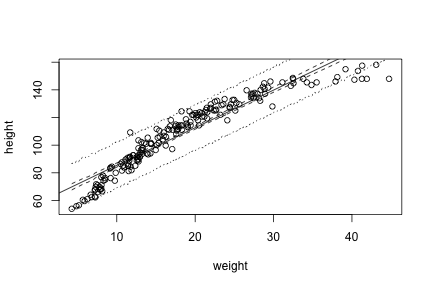
\includegraphics{pi-youth} \end{kframe}}
\end{knitrout}


\subsubsection{c}

Most concerned by the performance of the fit at low and high weights. 
In particular, the model underpredicts height at the upper end of the weight range, and overpredicts at lower end of the range.
I expect these poblems arise because the linear model cannot accommodate the biological reality of growth and development; the amount of energy (weight) allocated height may change over development. 
Further, height levels off at low weights.

To accommodate biological reality, I would use a model where growth has  non-linear relationship with weight.
Maybe a sinusoid: non-growth development early, then even develoment/height, then leveling off to maintenance.
Would like to keep intercept at zero though

One could also transform the data\dots 


\subsection*{Problem 3}

Suppose a colleague of yours, who works on allometry, glances at the homework problems just above. Your colleague exclaims, “That’s silly. Everyone knows that it’s only the logarithm of body weight that scales with height!”

(a) I want you to model the relationship between height (cm) and the natural logarithm of weight (log-kg). Use the entire Howell1 data frame, all 544 rows, adults and non-adults. Fit this model, using qua- dratic approximation:
\[h_i \sim Normal(\mu_i, \sigma), \mu_i =\alpha+\beta \log(w_i),\]

where hi is the height of individual i and wi is the weight (in kg) of individual i. The function for computing a natural log in R is just log.

(b) Begin with this plot:
\begin{knitrout}
\definecolor{shadecolor}{rgb}{.97, .97, .97}{\color{fgcolor}\begin{kframe}
\begin{flushleft}
\ttfamily\noindent
\hlfunctioncall{plot}\hlkeyword{(}\hlsymbol{height}{\ }\hlkeyword{\urltilda{}}{\ }\hlsymbol{weight}\hlkeyword{,}{\ }\hlargument{data}{\ }\hlargument{=}{\ }\hlsymbol{Howell1}\hlkeyword{,}{\ }\hlargument{col}{\ }\hlargument{=}{\ }\hlfunctioncall{col.alpha}\hlkeyword{(}\hlstring{"slateblue"}\hlkeyword{,}\hspace*{\fill}\\
\hlstd{}{\ }{\ }{\ }{\ }\hlnumber{0.4}\hlkeyword{)}\hlkeyword{)}\mbox{}
\normalfont
\end{flushleft}
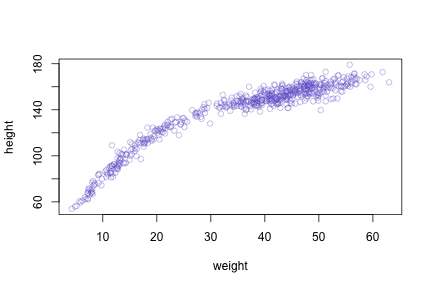
\includegraphics{all-data} \end{kframe}}
\end{knitrout}



Then use samples from the naive posterior of the model in (a) to su- perimpose on the plot (1) the predicted mean height as a function of weight, (2) the 95\% HPDI for the mean, and (3) the 95\% HPDI for predicted heights. The trick here lies in appreciating that the model was fit using log(weight) but that you must plot the predictions using raw weight as the horizontal axis. Remember that the opposite of log is exp.

\subsection*{Colophon}

\begin{knitrout}
\definecolor{shadecolor}{rgb}{.97, .97, .97}{\color{fgcolor}\begin{kframe}
\begin{flushleft}
\ttfamily\noindent
\hlfunctioncall{require}\hlkeyword{(}\hlsymbol{knitr}\hlkeyword{)}{\ }{\ }\hlcomment{\usebox{\hlnormalsizeboxhash}\usebox{\hlnormalsizeboxhash}\usebox{\hlnormalsizeboxhash}{\ }the{\ }package}\hspace*{\fill}\\
\hlstd{}\hlfunctioncall{knit}\hlkeyword{(}\hlstring{"/Users/jaime/PHD/stat-rethink/hw3ashander.Rnw"}\hlkeyword{)}{\ }{\ }\hlcomment{\usebox{\hlnormalsizeboxhash}\usebox{\hlnormalsizeboxhash}{\ }to{\ }run}\mbox{}
\normalfont
\end{flushleft}
\end{kframe}}
\end{knitrout}



\end{document}
